\documentclass[11pt]{article}
\usepackage{graphicx} 
\usepackage{natbib}
\title{Hausaufgabe 1 \\ Flussprobem}
\author{Jan Niklas Hollenbeck \\ und \\ Marco Leeske}
\date{\today}
\begin{document}
\maketitle
\newpage
\begin{abstract}
Dies Ist ein Abstract. Dies Ist ein Abstract.Dies Ist ein Abstract.Dies Ist ein Abstract.Dies Ist ein Abstract.Dies Ist ein Abstract.Dies Ist ein Abstract.Dies Ist ein Abstract.Dies Ist ein Abstract.Dies Ist ein Abstract.Dies Ist ein Abstract.Dies Ist ein Abstract.Dies Ist ein Abstract.Dies Ist ein Abstract.Dies Ist ein Abstract.Dies Ist ein Abstract.Dies Ist ein Abstract.Dies Ist ein Abstract.Dies Ist ein Abstract.Dies Ist ein Abstract.
\end{abstract}

\section{Einleitung}
\subsection{Problem}
Das Flussproblem ist ein mathematisches Problem zur Findung von maximalen Durchsatz in Netzwerken.
\subsection{Graph}
Diese Netzwerke zeichnen sich durch Ihre Richtung aus. Durch ihn fließt von der Quelle zur Senke immer eine Menge an Einheiten. Diese Können Liter, Autos oÄ. sein. In Figure \ref{fig:Graph1} Sieht man die Senke Auf der linken Seite gekennzeichnet durch "S".

\citet{Testref}blasdf asersdf aewras dfaer

\begin{figure}[h] 
  \centering
     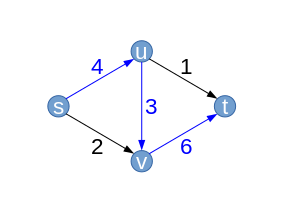
\includegraphics[width=0.48\textwidth]{graph1} 
  \caption{Bild eines Netzwerk-Graphens}
  \label{fig:Graph1}
\end{figure}
\bibliography{test.bib}
\bibliographystyle{plainnat}
\end{document}
